\documentclass[12pt]{article}

%%%%%%%%%%%%%%%%%%%%%%%%%%%%%%%%%%%%%%%%%%%%%%%%%%%%%%%%%%%%%%%%%%%%%%%%%%%%%%%%%%%%%%%%%%%%%%%%%%%%
% Math
\usepackage{fancyhdr} 
\usepackage{amsfonts}
\usepackage{amsmath}
\usepackage{amssymb}
\usepackage{amsthm}
%\usepackage{dsfont}

%%%%%%%%%%%%%%%%%%%%%%%%%%%%%%%%%%%%%%%%%%%%%%%%%%%%%%%%%%%%%%%%%%%%%%%%%%%%%%%%%%%%%%%%%%%%%%%%%%%%
% Macros
\usepackage{calc}

%%%%%%%%%%%%%%%%%%%%%%%%%%%%%%%%%%%%%%%%%%%%%%%%%%%%%%%%%%%%%%%%%%%%%%%%%%%%%%%%%%%%%%%%%%%%%%%%%%%%
% Commands and Custom Variables	
\newcommand{\problem}[1]{\hspace{-4 ex} \large \textbf{Problem #1} }
\let\oldemptyset\emptyset
\let\emptyset\varnothing
\newcommand{\norm}[1]{\left\lVert#1\right\rVert}
\newcommand{\sint}{\text{s}\kern-5pt\int}
\newcommand{\powerset}{\mathcal{P}}
\renewenvironment{proof}{\hspace{-4 ex} \emph{Proof}:}{\qed}
\newcommand{\RR}{\mathbb{R}}
\newcommand{\NN}{\mathbb{N}}
\newcommand{\QQ}{\mathbb{Q}}
\newcommand{\ZZ}{\mathbb{Z}}
\newcommand{\CC}{\mathbb{C}}
\renewcommand{\Re}{\operatorname{Re}}
\renewcommand{\Im}{\operatorname{Im}}


%%%%%%%%%%%%%%%%%%%%%%%%%%%%%%%%%%%%%%%%%%%%%%%%%%%%%%%%%%%%%%%%%%%%%%%%%%%%%%%%%%%%%%%%%%%%%%%%%%%%
%page
\usepackage[margin=1in]{geometry}
\usepackage{setspace}
%\doublespacing
\allowdisplaybreaks
\pagestyle{fancy}
\fancyhf{}
\rhead{Shaw \space \thepage}
\setlength\parindent{0pt}

%%%%%%%%%%%%%%%%%%%%%%%%%%%%%%%%%%%%%%%%%%%%%%%%%%%%%%%%%%%%%%%%%%%%%%%%%%%%%%%%%%%%%%%%%%%%%%%%%%%%
%Code
\usepackage{listings}
\usepackage{courier}
\lstset{
	language=Python,
	showstringspaces=false,
	formfeed=newpage,
	tabsize=4,
	commentstyle=\itshape,
	basicstyle=\ttfamily,
}

%%%%%%%%%%%%%%%%%%%%%%%%%%%%%%%%%%%%%%%%%%%%%%%%%%%%%%%%%%%%%%%%%%%%%%%%%%%%%%%%%%%%%%%%%%%%%%%%%%%%
%Images
\usepackage{graphicx}
\graphicspath{ {images/} }
\usepackage{float}

%tikz
\usepackage[utf8]{inputenc}
\usepackage{pgfplots}
\usepgfplotslibrary{groupplots}

%%%%%%%%%%%%%%%%%%%%%%%%%%%%%%%%%%%%%%%%%%%%%%%%%%%%%%%%%%%%%%%%%%%%%%%%%%%%%%%%%%%%%%%%%%%%%%%%%%%%
%Hyperlinks
%\usepackage{hyperref}
%\hypersetup{
%	colorlinks=true,
%	linkcolor=blue,
%	filecolor=magenta,      
%	urlcolor=cyan,
%}

\begin{document}
	\thispagestyle{empty}
	
	\begin{flushright}
		Sage Shaw \\
		m566 - Spring 2018 \\
		\today
	\end{flushright}
	
{\large \textbf{HW - Chapter 7}}\bigbreak

\problem{5 (a)} From the text, the eigenvalues of the matrix $A$ are 
$$\lambda_{l,m} = 4 - 2 \big( \cos(l \pi h) + \cos(m \pi h) \big)$$
where $1 \leq l,m \leq N$ and $h = \frac{1}{N+1}$. Note that these are all positive values, and thus $A$ is not just symmetric, but SPD. Then $\norm{A}_2 = \rho(A) = \lambda_{\text{max}}$ and $\norm{A^{-1}}_2 = \rho(A^{-1}) = \lambda_{\text{min}}$. \break

Since the argument to each Cosine function in the formula above is between $0$ and $\pi$ we know that it will be increasing as each $l$ and $m$ increase. Thus the largest eigenvalue will be given by the largest values of $l$ and $m$ and the smallest eigenvalue will be given by the smallest values of $l$ and $m$. Thus 
\begin{align*}
	\lambda_\text{max} & = 4 - 2 \big( \cos(N \pi h) + \cos(N \pi h) \big) \\
	& = 4 - 4 \cos\left(\frac{N }{N+1}\pi \right) \\
	\lambda_\text{min} & = 4 - 2 \big( \cos(1 \pi h) + \cos(1 \pi h) \big) \\
	& = 4 - 4 \cos\left(\frac{1 }{N+1}\pi \right)
\end{align*}
Due to symmetries of Cosine $\cos\left(\frac{N }{N+1}\pi \right) = -\cos\left(\frac{1 }{N+1}\pi \right)$ and we can rewrite
$$
\lambda_\text{max} = 4 + 4 \cos\left(\frac{1 }{N+1}\pi \right)
$$
Finally we find that the condition number of $A$ is given by
\begin{align*}
	\kappa(A) & = \left( 4 + 4 \cos\left(\frac{1 }{N+1}\pi \right) \right) 
		\left( 4 - 4 \cos\left(\frac{1 }{N+1}\pi \right) \right)^{-1} \\
	& = \frac{1 + \cos\left(\frac{1 }{N+1}\pi \right)}{ 1 - \cos\left(\frac{1 }{N+1}\pi \right)} \\
	& = \cot^2\left(\frac{\pi }{2(N+1)} \right)
\end{align*}


As $N$ gets large, the numerator approaches $2$ and the denominator approaches $0$, thus the condition number gets large. We can verify this by using Taylor Series approximations
\begin{align*}
	\frac{1 + \cos(x)}{ 1 - \cos(x)} & \approx \frac{1 + 1 - \frac{x^2}{2}}{1 - 1 + \frac{x^2}{2}} \\
	& = \frac{2 - \frac{x^2}{2}}{\frac{x^2}{2}} \\
	& = \frac{4}{x^2} - 1 \\
	\kappa(A) & \approx \left( \frac{2}{\frac{1}{N+1}\pi} \right)^2 \\
	& = \left( \frac{2N + 2}{\pi} \right)^2 \\
	& = \mathcal{O}(N^2) \\
	& = \mathcal{O}(n)
\end{align*}
As expected the condition number scales linearly with the discretization.

\problem{5 (b)} Since this problem asks to write code, it will be included here instead of in an appendix.
\begin{lstlisting}
def gen_A(N):
	n = N**2
	A = np.zeros((n,n))
	A += np.diag(4*np.ones(n), k=0)
	A += np.diag(-1*np.ones(n-1), k=1)
	A += np.diag(-1*np.ones(n-1), k=-1)
	A += np.diag(-1*np.ones(n-N), k=N)
	A += np.diag(-1*np.ones(n-N), k=-N)
	return A

def residual(x,b):
	n = len(x)
	N = int(np.sqrt(n))
	assert N**2 == n
	assert N>= 3
	r = np.zeros(n)
	r[0] = b[0] -4*x[0] + x[1] + x[N]
	for i in range(1, N):
		r[i] = b[i] + x[i-1] - 4*x[i] + x[i+1] + x[i+N]
	for i in range(N, n-N):
		r[i] = b[i] + x[i-N] + x[i-1] - 4*x[i] + x[i+1] + x[i+N]
	for i in range(n-N, n-1):
		r[i] = b[i] + x[i-N] + x[i-1] - 4*x[i] + x[i+1]
	r[-1] = b[-1] + x[-1-N] + x[-2] - 4*x[-1]
	return r

def p5b(N, tol):
	n = N**2
	x_old = np.ones(n)
	b = np.ones(n)/(N+1)
	r = residual(x_old, b)
	x_new = x_old + r/4
	while np.linalg.norm(r) > np.linalg.norm(b)*tol:
		r = residual(x_new, b)
		x_new, x_old = x_new + r/4, x_new
	print(x_new)
	#test the result by checking the 
	#	magnitude of the residual
	print(np.linalg.norm(b - np.dot(gen_A(N), x_new)))
	cond = (1+np.cos(np.pi/(N+1)))/(1-np.cos(np.pi/(N+1)))
	print('The condition number is %g.' % cond)
\end{lstlisting}

The output for this code ran with $N = 3$ and $\text{tol} = 10^{-8}$ is
\begin{lstlisting}
	>>> p5b(3, 10**-8)
	[0.23870482 0.31024097 0.3373494  
	0.39457832 0.41490964 0.39457832 
	0.3373494  0.31024097 0.23870482]
	6.08489253834842e-09
	The condition number is 5.82843.
\end{lstlisting}

\problem{5 (c)} The results for using the Jacobi method for $N = 2^l - 1$ are given below.
\begin{center}
	\begin{tabular}{|c|c|c|c|c|}
		\hline
		$l$&$N$&$n$&iterations required&$\kappa(A)$\\ \hline
		2&3&9&71&5.828427124746191\\ \hline
		3&7&49&333&25.274142369088175\\ \hline
		4&15&225&1389&103.08686891981736\\ \hline
		5&31&961&5618&414.3450622319052\\ \hline
	\end{tabular}
\end{center}

\begin{figure}[H]
	\caption{n versus K(A)}
	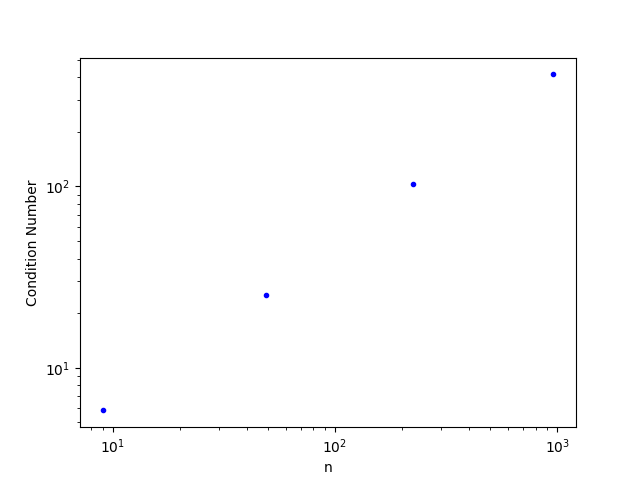
\includegraphics[width=1\textwidth]{hwch7_figure_1}
	\label{5c1}
	\centering
\end{figure}

\begin{figure}[H]
	\caption{iteration vs norm of the residual}
	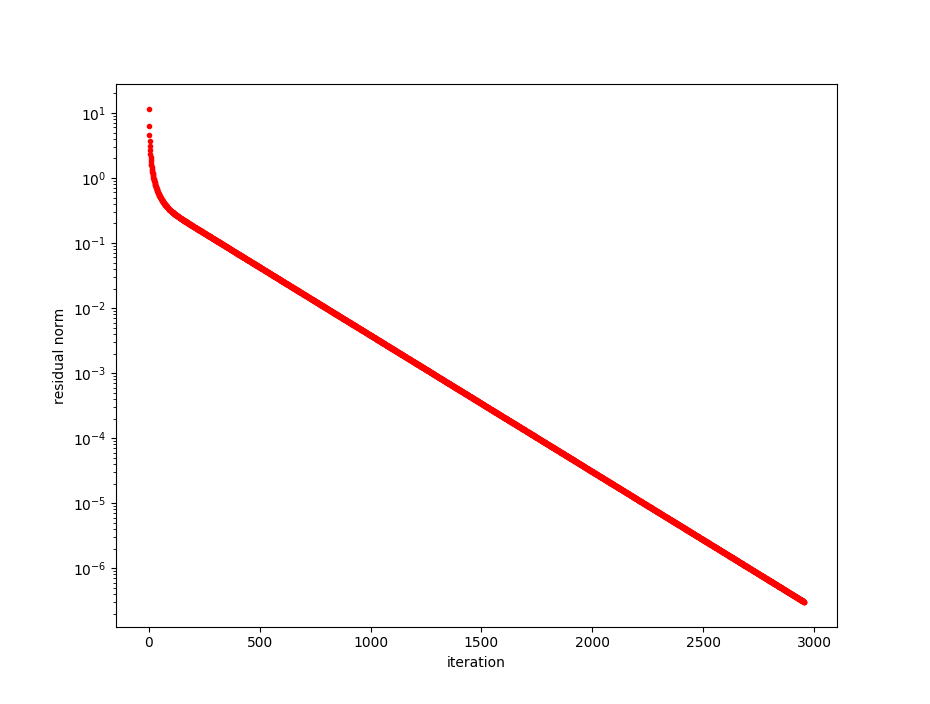
\includegraphics[width=1\textwidth]{hwch7_figure_2}
	\label{5c2}
	\centering
\end{figure}

As expected the condition number scales linearly with $n$ and it takes roughly a constant number of iterations to reduce the norm of the residual by a factor. From the table it seems that the number of iterations required scales linearly with $n$. 

\problem{9 (a)} Using the iteration scheme $x_{k+1} = x_k + \alpha(b-Ax_k)$ the splitting associated would be $A= M-N$ where $M = \alpha I$. Then 
\begin{align*}
	T & = I - M^{-1}A \\
	& = I - \frac{1}{\alpha}IA \\
	& = I - \frac{1}{\alpha}A
\end{align*}

\problem{9 (b)} We have a theorem that says that a Stationary Method converges if and only if the spectral radius is less than one. Suppose that $A$ is SPD with eigenvalues $\lambda_1 > \lambda_2 > ... > \lambda_n > 0$. Then $T$ is symmetric. Suppose that $x_k$ is an eigenvector corresponding to the eigenvalue $\lambda_k$. Then
\begin{align*}
	Tx_k & = Ix_k - \frac{1}{\alpha}Ax_k \\
	& = x_k - \frac{\lambda_k}{\alpha}x_k \\
	& = \left(1-\frac{\lambda_k}{\alpha} \right)x_k
\end{align*}
Thus each eigenvector of $A$ is also an eigenvector of $T$ corresponding to an eigenvalue of $\left(1-\frac{\lambda_k}{\alpha} \right)$. Since $T$ is symmetric, $\rho(T) = \max\limits_k \{ \left\vert 1-\frac{\lambda_k}{\alpha} \right \vert \}$. In order for the method to converge, we require that this value be less than 1. \bigbreak

Suppose that $\alpha < 0$. Then we get that 
$$
-\frac{\lambda_1}{\alpha} > -\frac{\lambda_2}{\alpha} > ... > -\frac{\lambda_n}{\alpha} > 0
$$
$$
1-\frac{\lambda_1}{\alpha} > 1-\frac{\lambda_2}{\alpha} > ... > 1-\frac{\lambda_n}{\alpha} > 1
$$
and our iterations fail to converge.
Suppose that $\alpha > 0$. Then
$$
1-\frac{\lambda_1}{\alpha} < 1-\frac{\lambda_2}{\alpha} < ... < 1-\frac{\lambda_n}{\alpha} < 1
$$
As long as $-1 < 1-\frac{\lambda_1}{\alpha}$ this will converge. Solving for $\alpha$ we get our final result: \bigbreak

The iteration $x_{k+1} = x_k + \alpha(b-Ax_k)$ will converge if and only if $\frac{\lambda_1}{2} < \alpha$ where $\lambda_1$ is the largest eigenvalue of the SPD matrix $A$. \bigbreak

To maximize the rate of convergence we need to minimize the spectral radius. This is made simpler by noting that 
$$
\rho(T) = \max \left\{  \left\vert 1-\frac{\lambda_1}{\alpha} \right\vert, \left\vert 1 - \frac{\lambda_n}{\alpha}\right\vert \right \}
$$
since the eigenvalues are indexed in decreasing magnitude. Suppose that $\alpha > \lambda_1$. Then 


\end{document}
